\chapter{Module Views}

\section{Global Module View}

\begin{figure}[h]
    \centering
    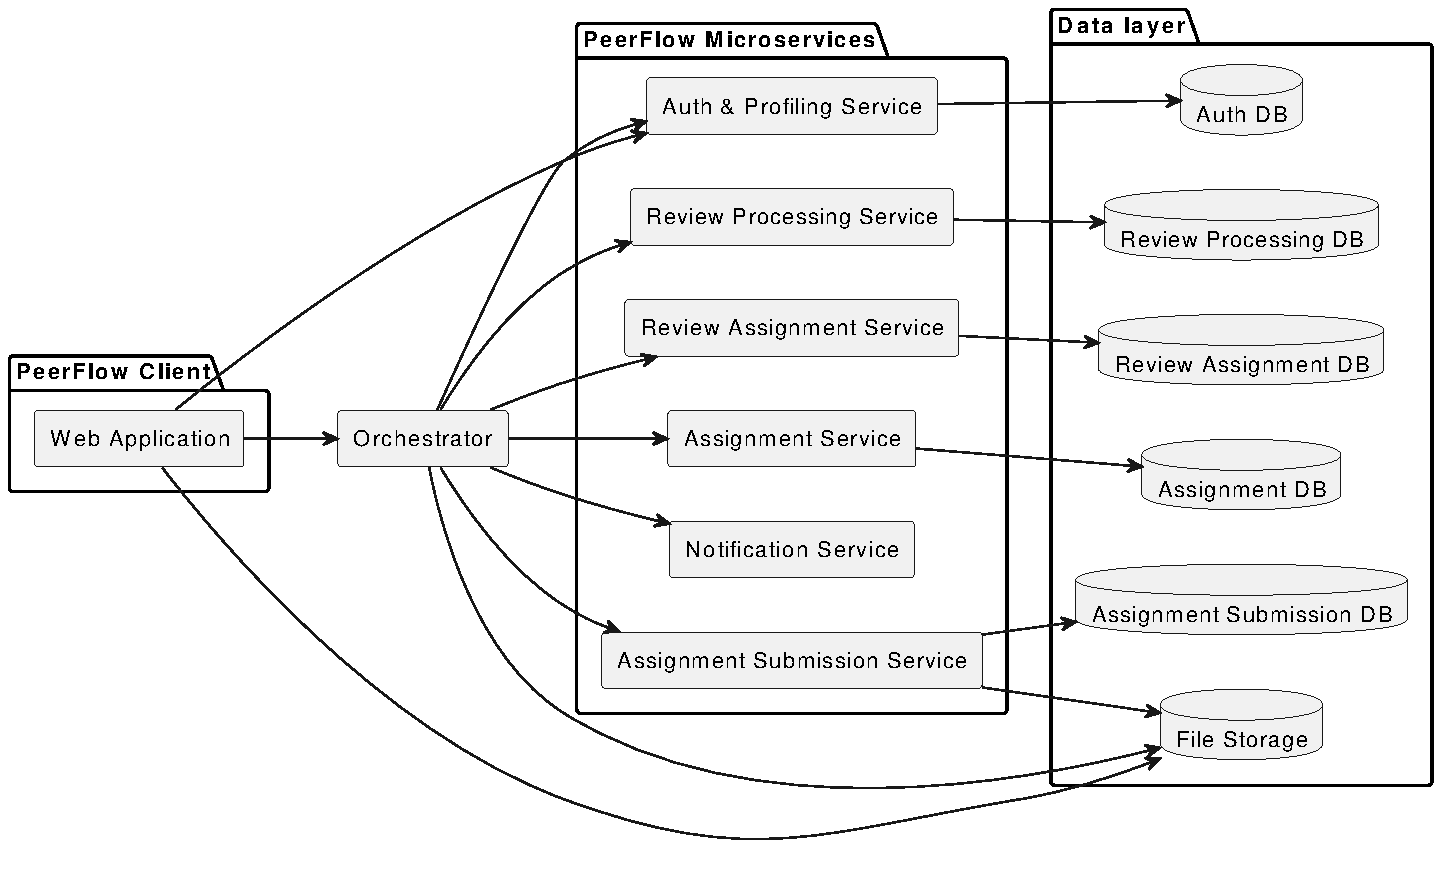
\includegraphics[width=0.9\linewidth]{Architettura/imgs/globalmoduleview.pdf}
    \caption{Global module view of PeerFlow.}
    \label{fig:moduleViewGlobal}
\end{figure}


\subsection{Elements}

\begin{enumerate}
    \item \textbf{Web Application}\label{def:WebApplication} 
    
    This component serves as a monolithic front-end application that Students and Teachers may use to access the system’s services. This component directly interacts with the Auth \& Profiling Service for authentication purposes; for all the other functionalities, this component interfaces with the Orchestrator service. Furhermore, it can ask for files directly to the FileStorage, which exposes a read-public HTTP API. 
    
    \item \textbf{Auth \& Profiling Service}\label{def:AuthProfilingService}
    
    This component exposes a REST API that allows users to sign up, log in, create, and refresh JWT tokens, and check the existence of users.
    \item \textbf{Assignment Service}\label{def:AssignmentService} 
    
    This component exposes a REST API that allows Teachers to create assignments within the course (specifying Students) and to edit them.
    \item \textbf{Assignment Submission Service}\label{def:AssignmentSubmissionService} 
    
    This component exposes a REST API that allows Students to submit their work (mandatory text and optional files) for the assignment.
    \item \textbf{Review Assignment Service}\label{def:ReviewAssignmentService} 
    
    This component exposes a REST API that allows Teachers to issue a Peer Review assignment for the students in the assignment (either manually or automatically specifying pairings).
    \item \textbf{Review Processing Service}\label{def:ReviewProcessingService} 
    
    This component exposes a REST API that allows Students to submit their reviews for the assignments they have been assigned to.
    \item \textbf{Notification Service}\label{def:NotificationService} 
    
    This service exposes a REST API that allows to send email notification to the users of the system.
    \item \textbf{Orchestrator}\label{def:Orchestrator} 
    
    This service exposes a REST API that the front-end application uses to interact with the system’s services. It acts as an intermediator capable of integrating more services, also exposing them to the final user as a single web endpoint.
    \item \textbf{File Storage Service}\label{def:FileStorageService} 
    
    This service exposes a REST API that manages files in an efficient and scalable way.
\end{enumerate}
\begin{justify}
   Each service (elements 1-7) has its own database istance, which is compliant with the microservice architecture. Data structures are described in the dedicated section. 
\end{justify}

\subsection{Rationale}

\begin{justify}
    The architectural design for PeerFlow, centered around a Microservices Architecture orchestrated by a dedicated orchestrator, addresses the core requirements and challenges of building a scalable, maintainable, and robust peer review system for MOOC environments.
\end{justify}

\subsubsection{Microservices Architecture}

\begin{justify}
    The adoption of a Service-Oriented/Microservices Architecture is a direct response to several key requirements and assumptions:
\end{justify}
\begin{itemize}
    \item \textbf{Scalability and High Availability:} PeerFlow "will be designed to support a large and highly variable number of users, typical of MOOC environments like Coursera or Udacity" and its architecture "will be based on a Service Oriented/Microservices Architecture approach, to ensure horizontal scalability, high availability, and low latency." Microservices support horizontal scalability by allowing individual services to be scaled independently based on their load. For instance, if there is a peak in assignment submissions, only the \hyperref[def:AssignmentSubmissionService]{Assignment Submission Service} needs to scale up, not the entire application. Similarly, high availability is achieved because the failure of one service (e.g., \hyperref[def:ReviewProcessingService]{Review Processing Service} as per \req{QA-AV-1} scenario) does not necessarily bring down the entire system, thanks to isolation and independent deployment.
    \item \textbf{Modifiability and Maintainability:} The non-functional requirements emphasize modifiability. For example, adding a new mandatory field to the student data model (\req{QA-MO-01}) or a new submission file type (\req{QA-MO-2}) is expected to be completed within a short timeframe with localized changes. A microservices approach ensures that changes have to be made to specific services, reducing the risk of introducing bugs in unrelated parts of the system and allowing for faster development cycles.
    \item \textbf{Technology Heterogeneity (Implied):} While not explicitly stated as a requirement, microservices allow for different technologies to be used for different services, optimizing each service for its specific function. This flexibility enhances future adaptability and leverages specialized tools.
    \item \textbf{Independent Deployment:} The Deployability non-functional requirements, such as deploying a bug fix to a specific service (\req{QA-DE-1}) or rolling back a malfunctioning service (\req{QA-DE-2}), are directly supported by the independent deployability of microservices. This minimizes downtime and risk during updates.
\end{itemize}

\subsubsection{Dedicated Microservices}

\begin{justify}
    Each service in the proposed architecture (\hyperref[def:AuthProfilingService]{Auth \& Profiling Service}, \hyperref[def:AssignmentService]{Assignment Service}, \hyperref[def:AssignmentSubmissionService]{Assignment Submission Service}, \hyperref[def:ReviewAssignmentService]{Review Assignment Service}, \hyperref[def:ReviewProcessingService]{Review Processing Service}, \hyperref[def:NotificationService]{Notification Service}, \hyperref[def:FileStorageService]{File Storage Service}) corresponds to a distinct functional area of the PeerFlow system, aligning with the "single responsibility principle" of microservices.
\end{justify}
\begin{itemize}
    \item \textbf{Auth \& Profiling Service:} Handles user authentication (sign-up, login, JWT tokens) and user profile management, directly addressing \req{FR-SYS-001} (two distinct user roles), \req{FR-SYS-002} (user authentication), and \req{FR-SYS-003} (new user sign-up). Its isolation ensures security concerns are centralized and managed effectively.
    \item \textbf{Assignment Service:} Manages the creation, modification, and viewing of assignments by teachers, addressing \req{FR-ASG-001}, \req{FR-ASG-002}, \req{FR-ASG-003}, \req{FR-ASG-004}. It also handles the listing of assignments for students (\req{FR-ASG-006}).
    \item \textbf{Assignment Submission Service:} Dedicated to handling student submissions, including text and file attachments (\req{FR-SUB-001}, \req{FR-SUB-002}, \req{FR-SUB-003}). Its separate nature allows for robust handling of potentially large file uploads and associated storage.
    \item \textbf{Review Assignment Service:} Manages the definition of rubrics (\req{FR-PRV-001}, \req{FR-PRV-002}, \req{FR-PRV-003}) and the initiation of the peer review process, including automatic or manual peer assignment (\req{FR-PRV-004}). This separation ensures that the complex logic of peer assignment is isolated.
    \item \textbf{Review Processing Service:} Focuses on the actual review process by students, including viewing assigned submissions and submitting reviews (\req{FR-REV-001}, \req{FR-REV-002}). This separation allows for efficient processing of review data.
    \item \textbf{Notification Service:} Handles sending email notifications to users (\req{FR-ASG-005}, \req{FR-PRV-005}). This service is designed for integrability, as indicated by scenario \req{QA-IN-1}.
    \item \textbf{File Storage Service:} Its inclusion is crucial for managing file attachments, as students must be able to submit file attachments (\req{FR-SUB-001}), view or download their own submitted work (\req{FR-SUB-002}), and modify their submitted work (\req{FR-SUB-003}). It provides a scalable and efficient way to handle binary data separately from relational databases.
\end{itemize}

\subsubsection{Orchestrator Service (API Gateway)}

\begin{justify}
    The \hyperref[def:Orchestrator]{Orchestrator} acts as an API Gateway, an essential pattern in microservices architectures:
\end{justify}
\begin{itemize}
    \item \textbf{Simplifies Client-Side Development:} The \hyperref[def:WebApplication]{Web Application} interacts with a single \hyperref[def:Orchestrator]{Orchestrator} endpoint for most functionalities, rather than needing to know and manage multiple microservice endpoints. This simplifies the front-end logic and reduces coupling between the UI and individual services.
    \item \textbf{Request Routing and Composition:} The \hyperref[def:Orchestrator]{Orchestrator} can route requests to the appropriate microservices and potentially compose responses from multiple services before sending them back to the client. This is crucial for functionalities that span multiple services (e.g., displaying assignment details that might involve data from \hyperref[def:AssignmentService]{Assignment Service} and \hyperref[def:AssignmentSubmissionService]{Assignment Submission Service}).
    \item \textbf{Cross-Cutting Concerns:} The \hyperref[def:Orchestrator]{Orchestrator} is an ideal place to handle cross-cutting concerns such as load balancing, caching, request logging, and potentially security (though authentication is handled by \hyperref[def:AuthProfilingService]{Auth \& Profiling Service}).
    \item \textbf{Enables Evolution:} Changes to backend microservices can be abstracted away from the client by modifying the \hyperref[def:Orchestrator]{Orchestrator}'s routing logic, ensuring backward compatibility for the \hyperref[def:WebApplication]{Web Application}.
    \item \textbf{Reduces Load on Assignment Submission Service during high peak times:} The ability of the \hyperref[def:Orchestrator]{Orchestrator} to directly interact with the \hyperref[def:FileStorageService]{File Storage Service} allows to lighten the load on the \hyperref[def:AssignmentSubmissionService]{Assignment Submission Service} and increase its throughput, therefore lowering the need to scale this service. This is compliant with the \req{QA-PE-3} requirement.
\end{itemize}

\subsubsection{Dedicated Databases per Service}

\begin{justify}
    Each microservice having its own database instance (Auth DB, Assignment DB, Review Assignment DB, Review Processing DB, Assignment Submission DB) is a crucial point of the microservices paradigm:
\end{justify}
\begin{itemize}
    \item \textbf{Loose Coupling and Data Independence:} This prevents services from being tightly coupled through a shared database, which is a common monolith anti-pattern. Each service can evolve its data schema independently without impacting others.
    \item \textbf{Data Consistency and Autonomy:} Each service is responsible for its own data, ensuring data consistency within its boundaries. This also allows different services to use different types of databases if optimal for their specific data needs.
    \item \textbf{Scalability:} Databases can be scaled independently along with their associated services, as seen in \req{QA-AV-2} (Scheduled Database Maintenance) where read operations can switch to a replica, and \req{QA-PE-3} (Submission Peak) where underlying storage infrastructure scales.
\end{itemize}

\subsubsection{Web Application (Client)}

\begin{justify}
    The \hyperref[def:WebApplication]{Web Application} serves as the user interface, providing accessibility via a web platform as required. Its interaction model is consistent with modern web development practices:
\end{justify}
\begin{itemize}
    \item \textbf{Direct Authentication Interaction:} The WebApp directly interacts with the \hyperref[def:AuthProfilingService]{Auth \& Profiling Service} for authentication. This is a common and secure pattern, as authentication is a critical first step.
    \item \textbf{Direct File Storage Interaction:} The WebApp directly interacts with the \hyperref[def:FileStorageService]{File Storage Service} for viewing and downloading submitted files directly on the UI. This is a common pattern, as file visualization is a function specific to the UI and it should not encumber the \hyperref[def:Orchestrator]{Orchestrator}.
    \item \textbf{Orchestrator for Other Functionalities:} For all other functionalities, the WebApp interacts with the \hyperref[def:Orchestrator]{Orchestrator}. This simplifies client-side development, leverages the \hyperref[def:Orchestrator]{Orchestrator}'s routing capabilities, and allows the backend architecture to evolve more independently of the frontend.
\end{itemize}
\begin{justify}
    In summary, the chosen architecture effectively leverages the benefits of microservices — scalability, modifiability, independent deployment, and resilience—to meet the complex and evolving demands of a peer review system for large-scale online learning environments. The \hyperref[def:Orchestrator]{Orchestrator} acts as a crucial unifying layer, simplifying client interactions and managing the distributed nature of the system.
\end{justify}
\clearpage

\section{Data View}

\begin{figure}[h]
    \centering
    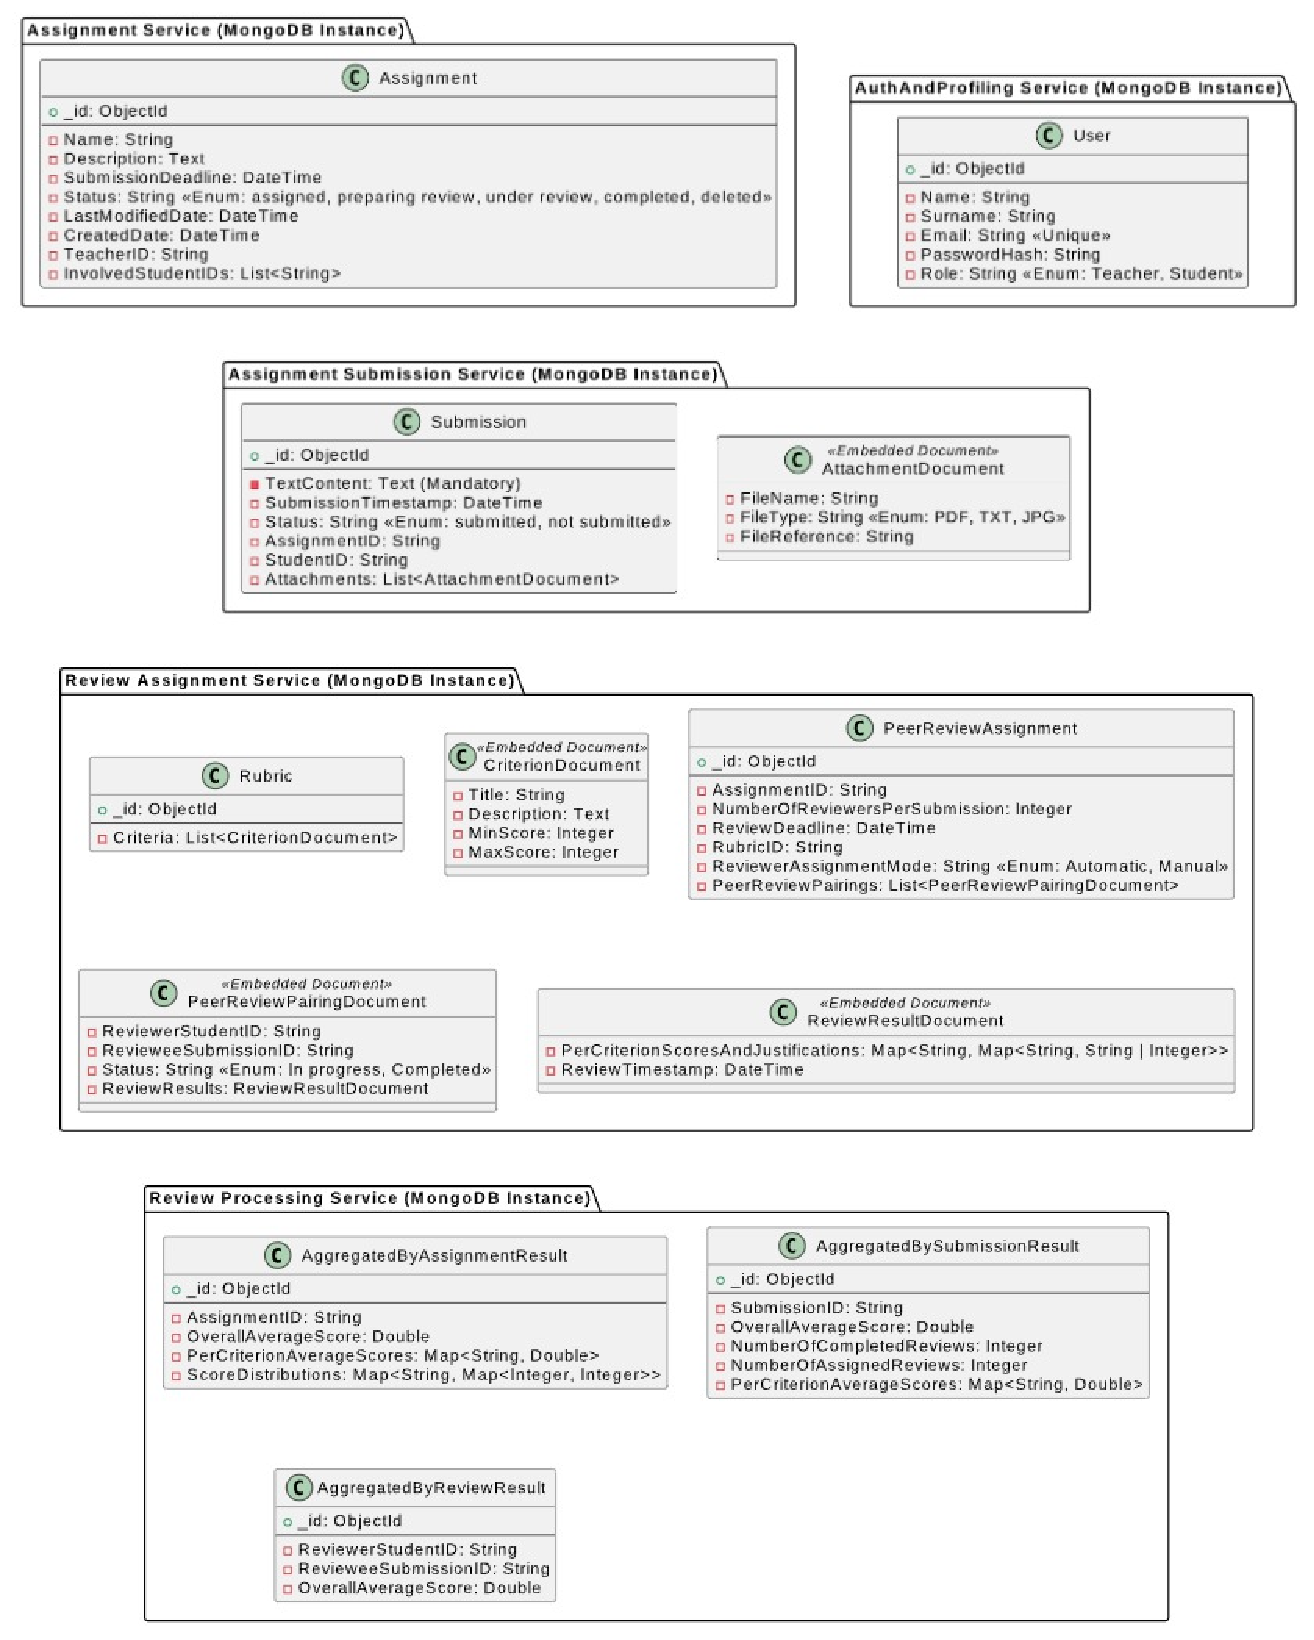
\includegraphics[width=0.9\linewidth]{Architettura/imgs/dataview.pdf}
    \caption{Data view of the system.}
    \label{fig:dataViewGlobal}
\end{figure}

\begin{justify}
    This section details the data view of the system, which is implemented using MongoDB. The data model is designed to leverage MongoDB's document-oriented capabilities, emphasizing data embedding for efficient data retrieval and reduced complexity in data operations.
The data view is structured as follows:
\end{justify}


\begin{itemize}
    \item \textbf{Collections:} Each top-level entity, represented by a distinct box in the diagram without the \texttt{<<embedded document>>} stereotype, corresponds directly to a MongoDB collection. The fields listed within these entities define the schema for documents stored within their respective collections, specifying both field names and their corresponding data types.

    \item \textbf{Embedded Documents:} Entities explicitly labeled with the \texttt{<<embedded document>>} stereotype do not constitute separate MongoDB collections. Instead, they define the structure of sub-documents that are embedded within documents of other collections.
\end{itemize}

\begin{justify}
    Consider the \texttt{PeerReviewAssignment} entity. This entity maps to the \texttt{PeerReviewAssignment} MongoDB collection. Documents within this collection will encapsulate details pertinent to a peer review assignment, including fields such as \texttt{\_id} (a unique identifier), \texttt{AssignmentId}, \texttt{NumberOfReviewersPerSubmission}, \texttt{ReviewDeadline}, \texttt{RubricId}, and \texttt{ReviewAssignmentMode}.

    A key aspect of this document's structure is the \texttt{PeerReviewPairings} field. This field is designed as a list of embedded documents. The precise structure of each element within this list is dictated by the \texttt{PeerReviewPairingDocument} entity, which is marked as an \texttt{<<embedded document>>}. Consequently, each embedded document within the \texttt{PeerReviewPairings} list will contain fields defining a specific review pairing, such as \texttt{ReviewerStudentID}, \texttt{RevieweeSubmissionID}, \texttt{Status} (indicating the progress of the review), and \texttt{ReviewResults} (another embedded document detailing the review outcomes).
\end{justify}

\subsection{Rationale}

\begin{justify}
    The embedded document strategy is employed to maintain data locality, optimize query performance by reducing the need for explicit joins, and align with MongoDB’s best practices for data modeling. It allows for the retrieval of all relevant pairing information directly within the parent assignment document, enhancing data access efficiency.
\end{justify}
